\documentclass[12pt]{article}
\usepackage{cmap}
\usepackage[T2A]{fontenc}
\usepackage[utf8]{inputenc}
\usepackage[russian]{babel}
\usepackage{tempora}
\usepackage[
    paperwidth=960bp,
    paperheight=540bp,
    left=40bp,
    right=40bp,
    top=20bp,
    bottom=36bp,
    footskip=18bp
]{geometry}
\usepackage{graphicx}
\usepackage[table]{xcolor}
\usepackage{array,tabularx}
\usepackage{enumitem}
\usepackage{fancyhdr}
\usepackage[hidelinks]{hyperref}

\hypersetup{
    pdftitle={Разработка базы данных для поиска и организации досуга},
    pdfauthor={М. В. Козин},
    pdfsubject={Презентация курсовой работы по дисциплине <<Базы данных>>}
}
\pagestyle{fancy}
\fancyhf{}
\fancyfoot[R]{\fontsize{11}{13}\selectfont\color{gray}\thepage}
\renewcommand{\headrulewidth}{0pt}
\renewcommand{\footrulewidth}{0pt}
\setlength{\parindent}{0pt}
\setlength{\parskip}{10bp}
\setlength{\tabcolsep}{9bp}
\renewcommand{\arraystretch}{1.35}
\definecolor{tablehead}{gray}{0.85}
\newcolumntype{L}[1]{>{\raggedright\arraybackslash}p{#1}}
\newcolumntype{Y}{>{\raggedright\arraybackslash}X}
\setlist[itemize]{label=--,leftmargin=24bp,labelsep=10bp,itemsep=7bp,topsep=5bp,parsep=0pt}
\hyphenpenalty=10000
\exhyphenpenalty=10000
\emergencystretch=2em

\newcommand{\slidetitle}[1]{%
    {\centering\fontsize{28}{34}\selectfont\bfseries #1\par}%
    \vspace{12bp}%
}
\newenvironment{slide}[1]{\clearpage\slidetitle{#1}}{\par}

\begin{document}
\fontsize{20}{26}\selectfont
\thispagestyle{empty}

{\centering\fontsize{18}{23}\selectfont
МОСКОВСКИЙ ГОСУДАРСТВЕННЫЙ ТЕХНИЧЕСКИЙ УНИВЕРСИТЕТ\par
ИМЕНИ Н.~Э.~БАУМАНА\par
(НАЦИОНАЛЬНЫЙ ИССЛЕДОВАТЕЛЬСКИЙ УНИВЕРСИТЕТ)\par}

\vspace{82bp}
{\centering\fontsize{32}{40}\selectfont\bfseries
<<Разработка базы данных\par
для поиска и организации досуга>>\par}

\vfill
\textbf{Студент:} Козин~М.~В.\par
\textbf{Группа:} ИУ7-64Б\par
\textbf{Руководитель:} Назаренко~Н.~В.\par
\vspace{24bp}

\begin{slide}{Цель и задачи}
\textbf{Цель:} спроектировать и реализовать базу данных для поиска и организации досуга и приложение для взаимодействия с ней.

\vspace{9bp}
\textbf{Задачи:}
\begin{itemize}
    \item проанализировать предметную область и известные решения;
    \item определить требования, сущности и связи между ними;
    \item спроектировать БД, ограничения, роли и триггер; проверить соответствие~3НФ;
    \item выбрать средства реализации и разработать приложение;
    \item описать методы тестирования и проверить основные операции;
    \item исследовать время поиска мероприятий с индексом и без него.
\end{itemize}
\end{slide}

\begin{slide}{Диаграмма <<сущность-связь>>}
\centering
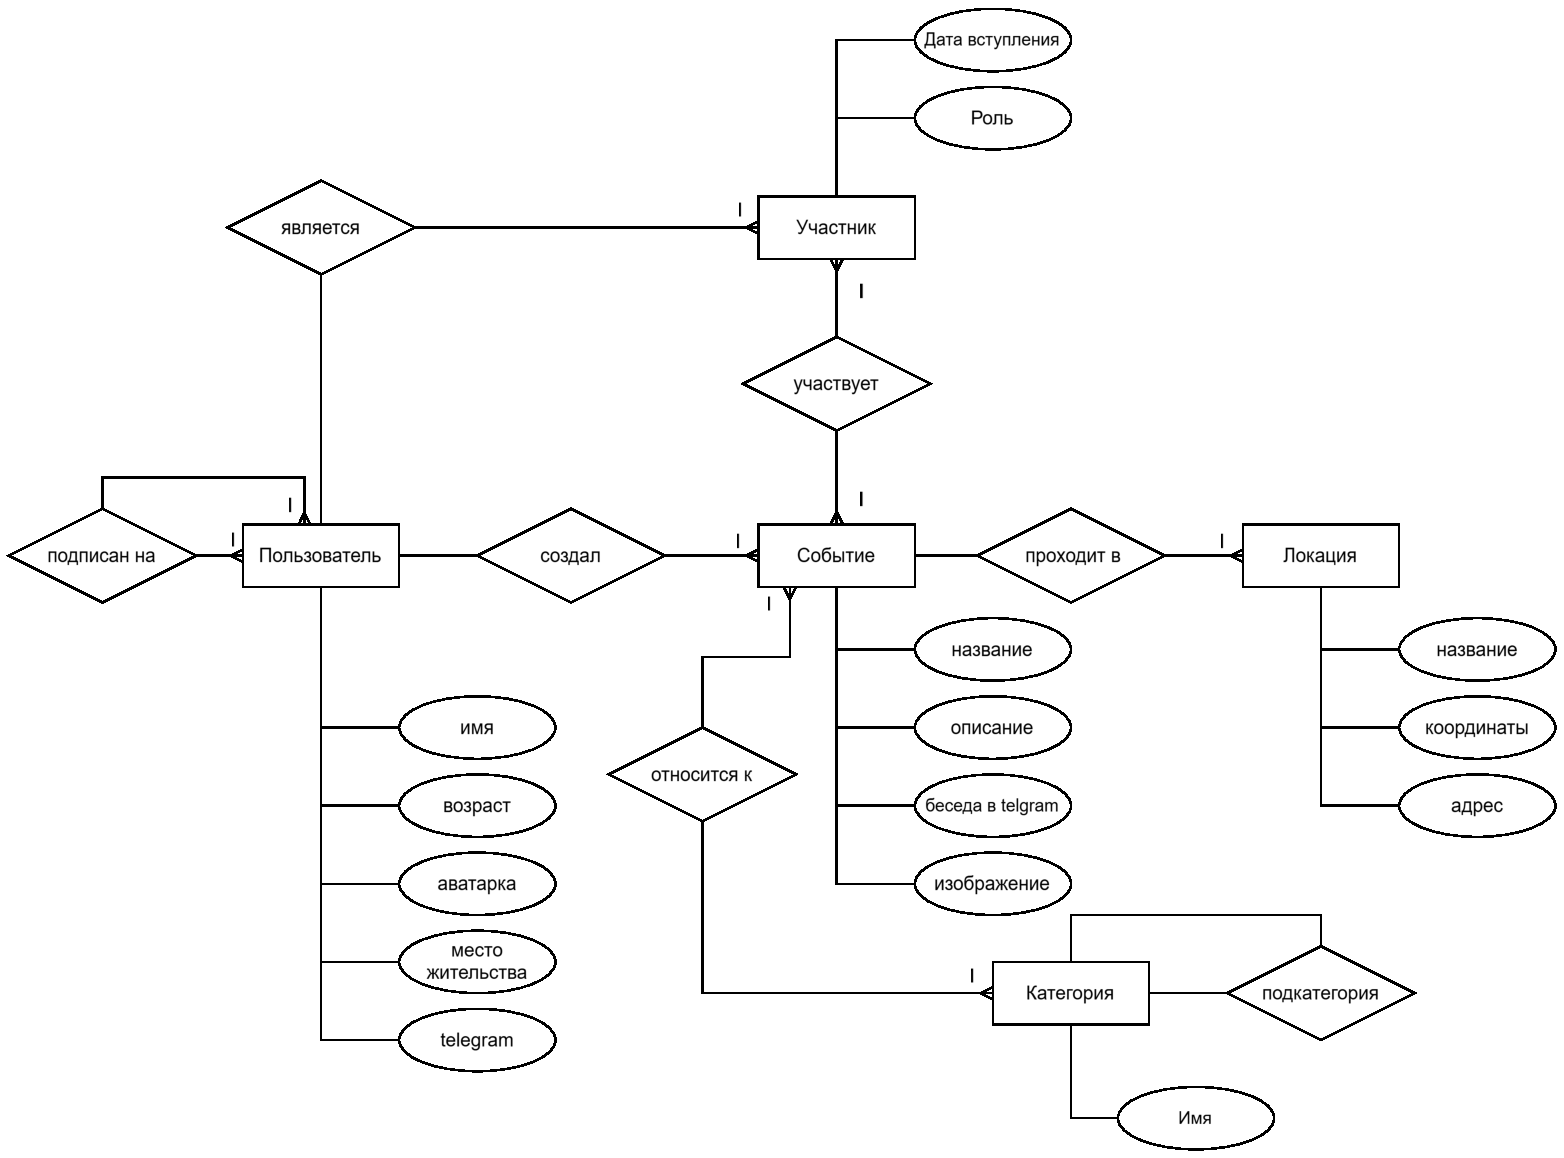
\includegraphics[height=421bp,width=\textwidth,keepaspectratio]{../images/ER.pdf}
\end{slide}

\begin{slide}{Выбор типа базы данных}
\begin{tabularx}{\textwidth}{|L{210bp}|Y|}
    \hline
    \rowcolor{tablehead}\textbf{Модель} & \textbf{Описание} \\
    \hline
    Иерархическая & Данные представлены деревом. Связи пользователей с несколькими мероприятиями требуют дополнительных ссылок или дублирования. \\
    \hline
    Документная & Объекты содержат вложенные данные или ссылки. Копирование сведений о пользователе усложняет их обновление. \\
    \hline
    \textbf{Реляционная} & \textbf{Данные представлены таблицами, связанными ключами. Участие и категории задаются отдельными отношениями.} \\
    \hline
\end{tabularx}

\vspace{12bp}
Выбрана \textbf{реляционная модель}: поиск выполняется отбором и соединением записей, рейтинг -- агрегированием оценок.
\end{slide}

\begin{slide}{Выбор системы управления базами данных}
\begin{tabularx}{\textwidth}{|L{270bp}|Y|Y|Y|}
    \hline
    \rowcolor{tablehead}\textbf{Критерий} & \textbf{PostgreSQL} & \textbf{MySQL} & \textbf{SQLite} \\
    \hline
    Внешние ключи & Да & Да & Требуют включения \\
    \hline
    Транзакции & Да & Да & Да \\
    \hline
    Триггеры & Да & Да & Да \\
    \hline
    Права на таблицы через GRANT и REVOKE & Да & Да & Нет \\
    \hline
\end{tabularx}

\vspace{16bp}
Выбрана \textbf{PostgreSQL~16}: она поддерживает необходимые ограничения, триггер и роли БД. Драйвер pgx обеспечивает доступ к ней из Go.
\end{slide}

\begin{slide}{Ролевая модель}
Приложение поддерживает три подключения к БД. Подключение выбирается в зависимости от роли пользователя.

\vspace{5bp}
\begin{tabularx}{\textwidth}{|L{210bp}|Y|Y|}
    \hline
    \rowcolor{tablehead}\textbf{Роль БД} & \textbf{Таблицы} & \textbf{Права} \\
    \hline
    Гость\newline (joinup\_guest) & event, location, image, category, event\_category, review & Чтение \\
    \hline
    Пользователь\newline (joinup\_user) & Все прикладные таблицы & Чтение, добавление, изменение и удаление \\
    \hline
    Администратор\newline (joinup\_admin) & Все прикладные таблицы & Все права на таблицы \\
    \hline
\end{tabularx}

\vspace{10bp}
Пользователь имеет права использования и чтения последовательностей, администратор -- все права на них.

Принадлежность мероприятия автору и полномочия администратора проверяются приложением.
\end{slide}

\begin{slide}{Интерфейс приложения}
\vspace{35bp}
\begin{minipage}[t]{0.49\textwidth}
    \centering
    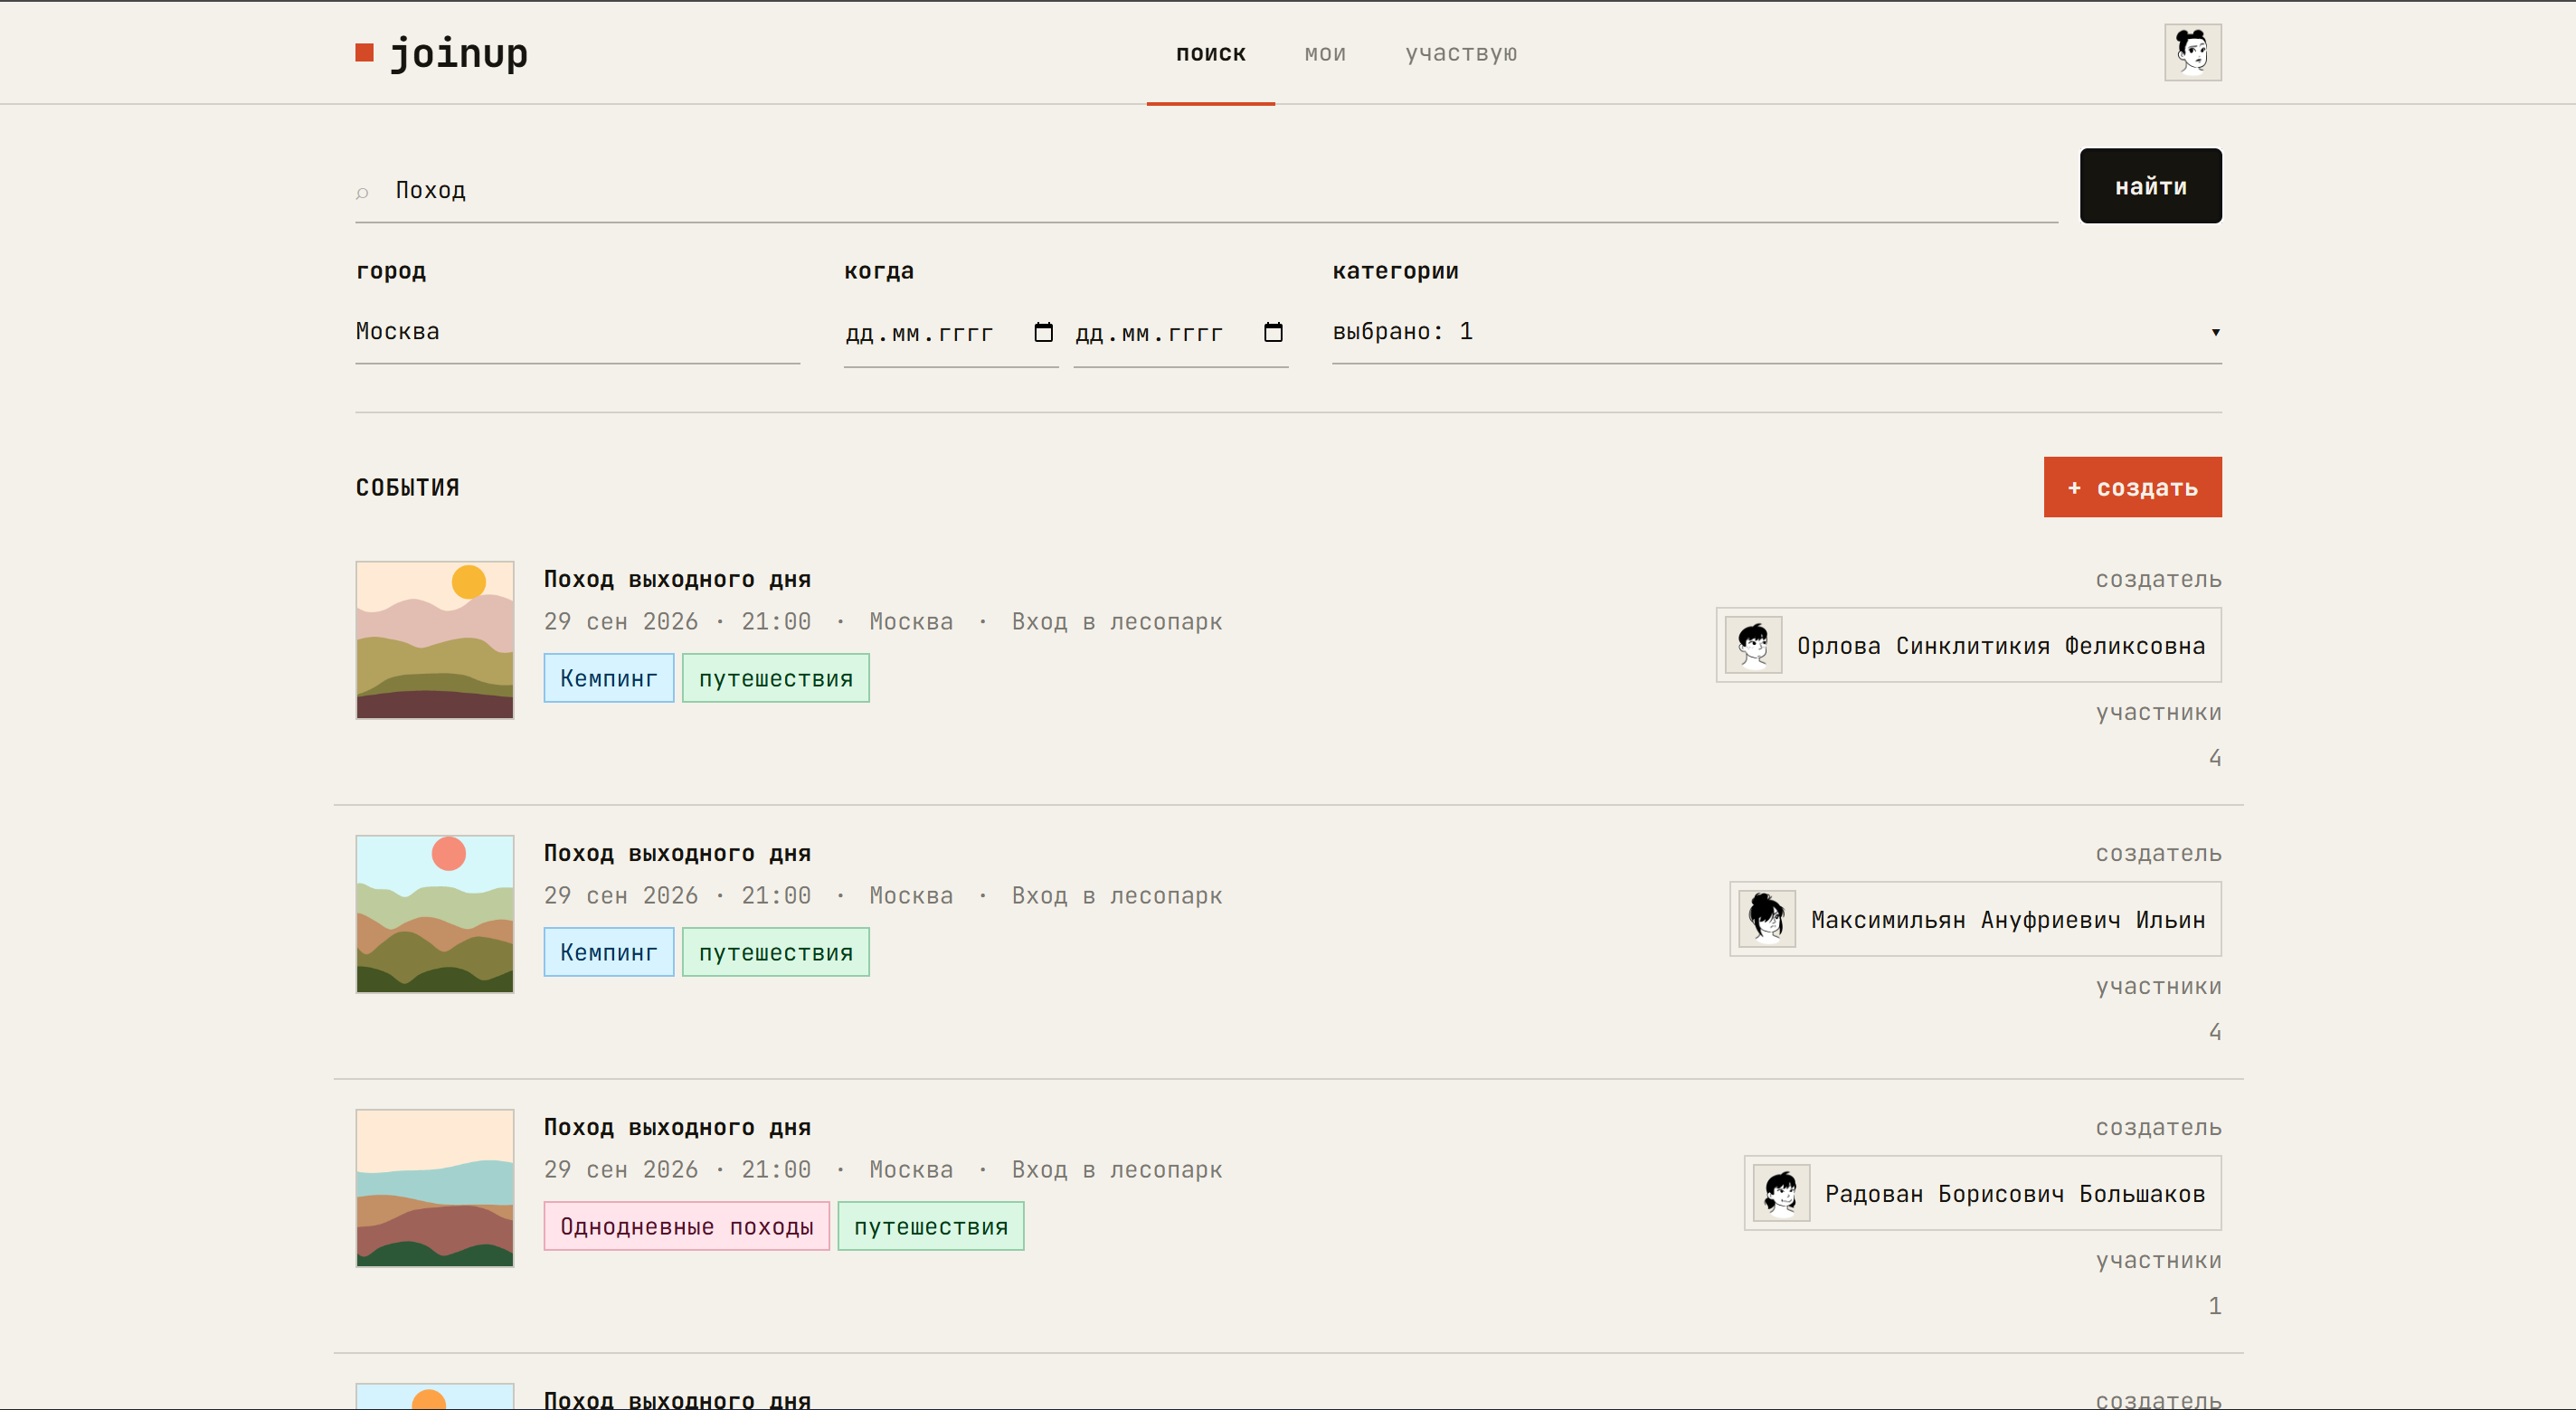
\includegraphics[trim=125bp 0bp 125bp 0bp,clip,width=\linewidth]{ui-search.png}\par
    \vspace{10bp}
    Поиск мероприятий с фильтрами
\end{minipage}\hfill
\begin{minipage}[t]{0.49\textwidth}
    \centering
    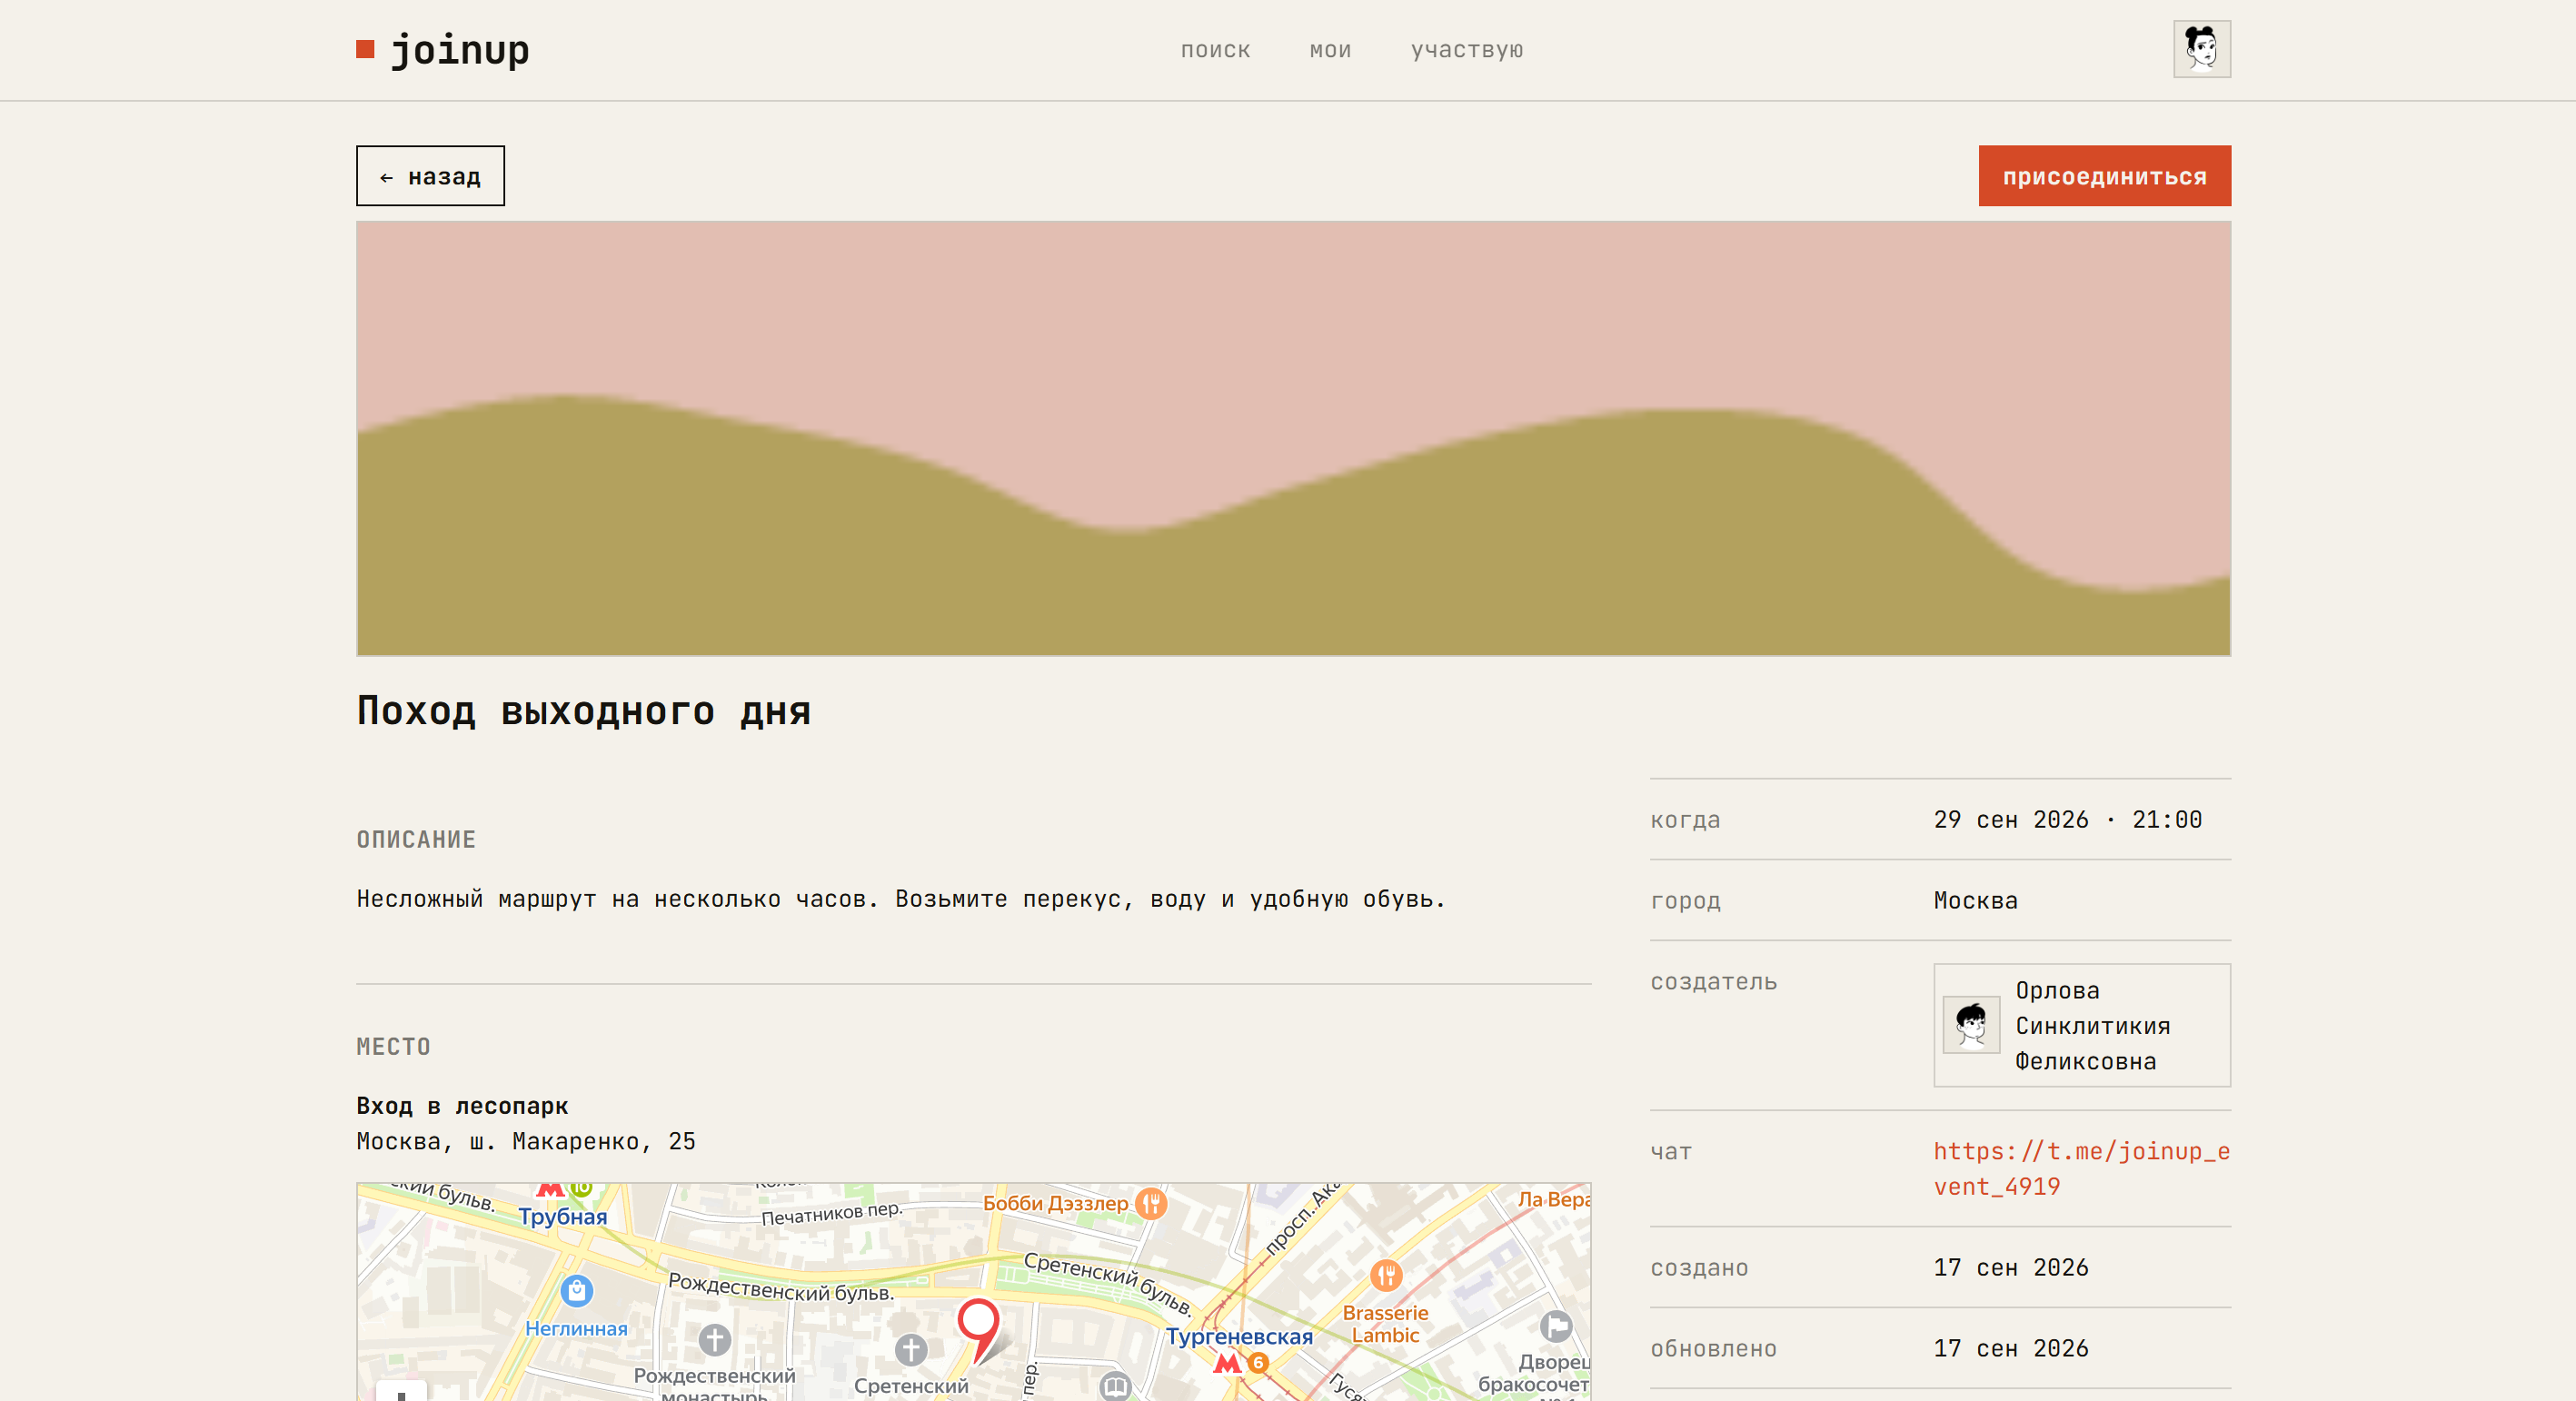
\includegraphics[trim=125bp 0bp 125bp 0bp,clip,width=\linewidth]{ui-event.png}\par
    \vspace{10bp}
    Карточка мероприятия
\end{minipage}
\end{slide}

\begin{slide}{Проведение исследования}
\begin{minipage}[c]{0.34\textwidth}
    \raggedright
    \setlength{\parskip}{10bp}
    \textbf{Влияние индекса на время поиска по городу и дате.}

    1000, 2000, 5000 и 10000~мероприятий.

    По 500~измерений каждого варианта; кеш БД прогрет.

    Для 10000~мероприятий:

    без индекса -- 4,905~мс;\newline
    с индексом -- 3,038~мс.

    \textbf{Время сократилось на~38\%.}
\end{minipage}\hfill
\begin{minipage}[c]{0.64\textwidth}
    \centering
    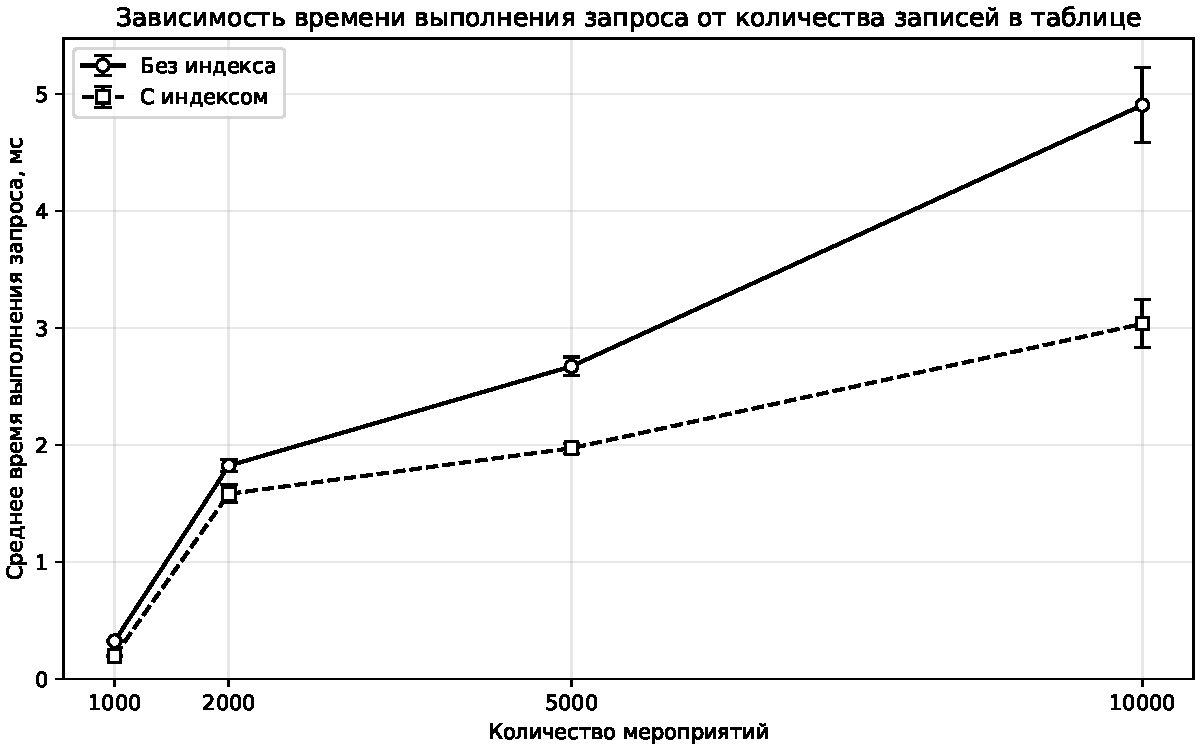
\includegraphics[width=\linewidth]{../app/scripts/index_chart.pdf}
\end{minipage}

\vspace{8bp}
Результат относится к основному SQL-запросу и условиям исследования.
\end{slide}

\begin{slide}{Заключение}
Цель работы достигнута: спроектированы и реализованы база данных для поиска и организации досуга и приложение JoinUp.

\vspace{9bp}
\textbf{Выполнены следующие задачи:}
\begin{itemize}
    \item проанализированы предметная область и известные решения;
    \item определены требования, сущности и связи между ними;
    \item спроектированы БД, ограничения, роли и триггер; обосновано соответствие~3НФ;
    \item выбраны средства реализации и разработано приложение;
    \item описаны методы тестирования; проверки дали ожидаемые результаты;
    \item исследовано время поиска мероприятий с индексом и без него.
\end{itemize}
\end{slide}

\end{document}
